% =====================================================================
% overleaf/chapters/06_Empirical_Evaluation.tex — LaTeX rendering of en/06_Empirical_Evaluation.md draft v0.4 (17 September 2026)
% Dernière mise à jour : 2026-09-21
% Chapter 6 of the paper, a \section of its own, to be inserted right after overleaf/chapters/05_Protocol.tex.
% This file DEFINES \label{sec:results}, referenced forward by overleaf/chapters/04_Evaluation.tex and
%   overleaf/chapters/05_Protocol.tex, and which resolved to ?? until this file existed. Keep the spelling.
% Forward reference: app:detail (appendix H) and app:unit (appendix I) are defined by overleaf/99_annexes.tex.
% Preamble additions:
%   \newcommand{\todo}[1]{\textbf{[#1]}}   % placeholder figures
% Figures: six, all PNG, all composed IN ENGLISH — four by scripts/analysis/plot_chapitre6.py, regenerated
%   on 2026-09-17, and the two of the unit audit by scripts/analysis/plot_audit_unitaire.py, 2026-09-21. Caption BELOW and a mandatory \Description{} (plain text, 2000 characters at most, not printed).
%   fig:scale and fig:residual are set as figure* (both columns): thirteen labelled rows, and six panels
%   respectively, are unreadable in a single column. fig:engineering and fig:distance fit \columnwidth.
%   FILES TO UPLOAD to the Overleaf project, flat, next to the .tex, as architecture_GAMA_Agents.jpg already is:
%   ch6_echelle.png, ch6_ingenierie.png, ch6_distance.png, ch6_residu.png, ch6_audit_modes.png
%   (sources in docs/paper/article/images/). ch6_audit_distance.png n'est plus appelée depuis le
%   2026-09-22 ; le script la produit toujours.
% Tables: four, caption ABOVE, booktabs (both loaded by aamas.cls). tab:scale (13 rows) and tab:engineering
%   (confidence intervals in the cells) are set as table* across both columns; tab:agreement and tab:unit fit one column.
% Numbers: the Markdown decimal comma becomes a decimal point, and the thousands separator a comma.
% Traceability: the "source:" comments live in the ../fr/ and ../en/ masters only. Do not carry them
%   over into this file when rendering a chapter into LaTeX (author's decision, 2026-09-21).
% Derived file: regenerate after every validated pass of en/06_Empirical_Evaluation.md.
% =====================================================================

\section{Empirical Evaluation}
\label{sec:results}

Section~\ref{sec:prompt} described four ways of deciding a travel mode from the same state. This section confronts them with the survey, on the cohort of 1{,}000 personas and the 3{,}154 scored decisions of the evaluated day.

Every result here bears on a couple: a language model and an arbitration instruction, carried by its system prompt and subject to the prohibitions of Section~\ref{sec:expert-prompt}, among them any numerical threshold. Engineering that prompt brings \texttt{gemini-3.5-flash-lite} 2.3 composite points closer to the survey distribution and \texttt{mistral-large-2512} 7.3 points closer, where cohort variation is of the order of 1.3 points. The carrier weighs as much as the instruction: submitted as it stands to a second model from the same provider, the variant tuned against \texttt{gemini-3.5-flash-lite} leaves 4.2 points between the two, more than it brings to the weaker of them. Of the three couples measured, one comes within a point and a half of the tabular ceiling, separable from two of the four reference methods and not separable from the other two, and that proximity of the margins covers a decision-by-decision disagreement that the tabular methods, among themselves, do not have.

\subsection{Thirteen deciders on the same scale}
\label{sec:scale}

The three readings defined in Section~\ref{sec:quantities} are published for every decider, in Table~\ref{tab:scale} and Figure~\ref{fig:scale}.

\begin{figure*}[tp]
  \centering
  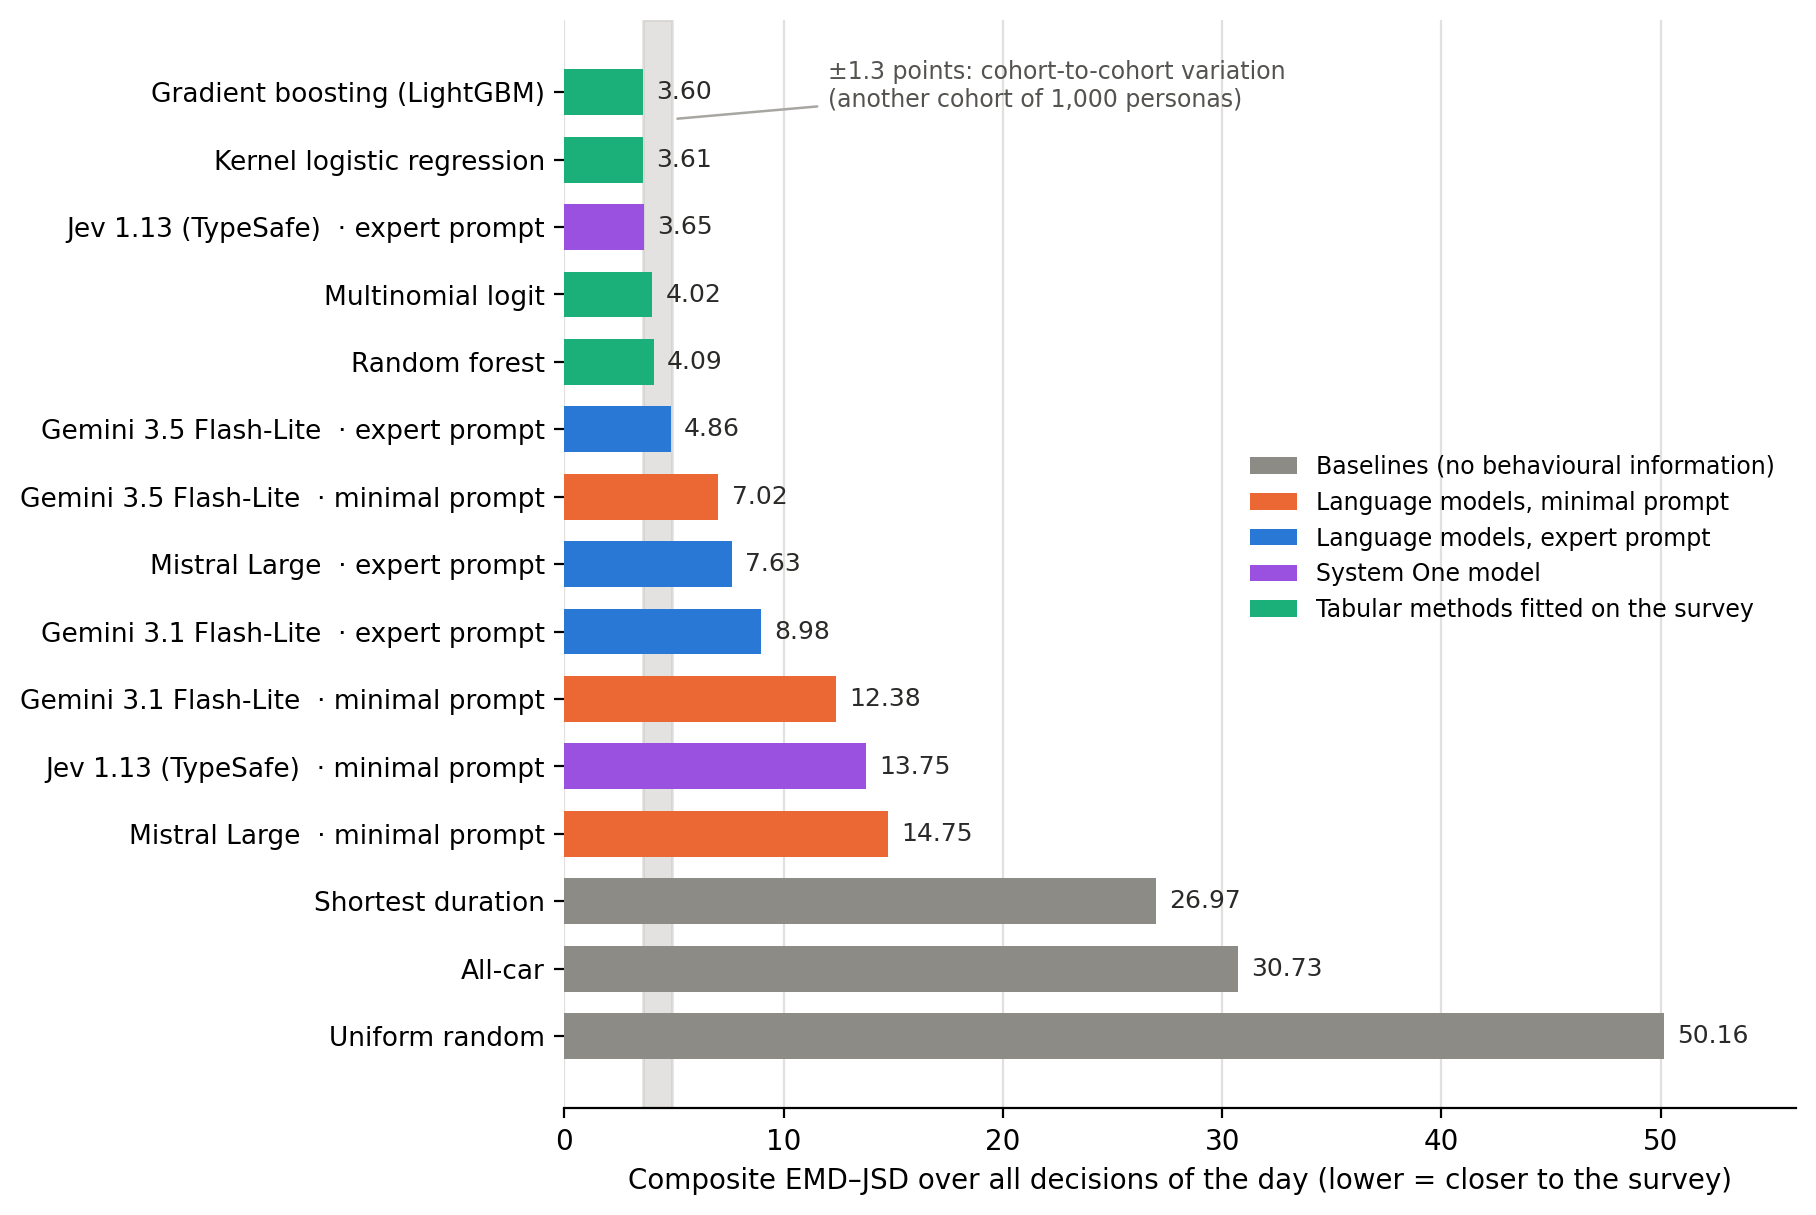
\includegraphics[width=\textwidth]{images/ch6_echelle.png}
  \caption{The thirteen deciders on the composite EMD--JSD axis, a factor of fourteen between the random floor and the best composite. Four groups separate on it: the floors from 27 to 50, the minimal prompt from 7.0 to 14.8, the expert prompt from 4.9 to 9.0, the four tabular methods from 3.60 to 4.09. The minimal prompt thus passes below the shortest-duration heuristic, at 27.0: the facts alone, with no arbitration instruction, already carry behavioural information. The grey band gives cohort variation, of the order of 1.3 points.}
  \label{fig:scale}
  \Description{A horizontal dot plot. The x axis is the composite EMD-JSD error, running from zero on the left to about fifty-five on the right; lower is better. Thirteen deciders are stacked as rows and coloured by group. At the far right, the three floors: uniform random draw at 50.2, all-car at 30.7, shortest duration at 27.0. In the middle, the three language models under the minimal prompt, mistral-large at 14.8, gemini-3.1-flash-lite at 12.4 and gemini-3.5-flash-lite at 7.0. Slightly to their left, the same three models under the expert prompt, gemini-3.1 at 9.0, mistral-large at 7.6 and gemini-3.5 at 4.9. At the far left, packed together between 3.6 and 4.1, the four tabular methods: gradient boosting, kernel logistic regression, the multinomial logit and the random forest. A vertical grey band of about 1.3 points in width marks cohort variation, the resolution below which two scores cannot be told apart.}
\end{figure*}

\begin{table*}[tp]
  \caption{The thirteen deciders on the three readings of the comparison protocol. The composite bears on every decision of the day, constrained trips included; the reading excluding single choice removes those where only one option existed; the L1 on global shares looks only at the four aggregate modal shares, with no stratification. In bold, the best score in each column; lower is better throughout.}
  \label{tab:scale}
  \begin{tabular}{llrrr}
    \toprule
    Group & Decider & Composite EMD--JSD & Excl.\ single choice & L1 global shares \\
    \midrule
    Floors     & Uniform random draw                            & 50.16 & 57.90 & 86.80 \\
               & All-car                                        & 30.73 & 28.41 & 58.00 \\
               & Shortest duration                              & 26.97 & 23.93 & 53.62 \\
    \midrule
    Minimal    & \texttt{mistral-large-2512}                    & 14.75 & 20.72 & 44.71 \\
    prompt     & \texttt{gemini-3.1-flash-lite}                 & 12.38 & 16.65 & 39.88 \\
               & \texttt{gemini-3.5-flash-lite}                 &  7.02 & 10.39 & 24.08 \\
    \midrule
    Expert     & \texttt{gemini-3.1-flash-lite}                 &  8.98 & 12.39 & 31.25 \\
    prompt     & \texttt{mistral-large-2512}                    &  7.63 & 12.27 & 26.64 \\
               & \texttt{gemini-3.5-flash-lite}                 &  4.86 &  6.86 & 13.85 \\
    \midrule
    Tabular    & Multinomial logit                              &  4.02 &  6.63 &  8.99 \\
    references & Random forest                                  &  4.09 &  5.81 & \textbf{5.28} \\
               & Kernel logistic regression                     &  3.61 & \textbf{5.61} &  6.69 \\
               & Gradient boosting (LightGBM)                   & \textbf{3.60} &  5.84 &  9.49 \\
    \bottomrule
  \end{tabular}
\end{table*}

\subsection{What prompt engineering moves}
\label{sec:engineering}

\begin{figure}[tbp]
  \centering
  
\includegraphics[width=\columnwidth]{images/ch6_ingenierie.png}
  \caption{What prompt engineering makes each model travel. The hollow circle is the minimal prompt, the filled circle the reference expert prompt, the squares two variants rewritten on the residuals of the cohort. The green band gives the interval of the four tabular methods. The three models start from different places, advance by different amounts, and one alone comes into contact with the band.}
  \label{fig:engineering}
  \Description{Three horizontal tracks, one per language model, over a common x axis of composite EMD-JSD error running from about three on the left to about fifteen on the right; lower is better. On each track a hollow circle marks the minimal prompt and a filled circle the expert prompt, joined by an arrow pointing left, that is towards lower error. The mistral-large-2512 track is the longest, from 14.8 down to 7.6. The gemini-3.1-flash-lite track runs from 12.4 down to 9.0. The gemini-3.5-flash-lite track is the shortest but ends furthest left, from 7.0 down to 4.9. Two square markers on the gemini-3.5 track sit further left still: variants tuned in sight of the evaluated cohort, shown apart as an in-sample upper bound. A vertical green band between 3.60 and 4.09 marks the interval of the four tabular methods; only the filled circle of gemini-3.5 comes into contact with it.}
\end{figure}

\begin{table*}[tp]
  \caption{Paired gain of the expert prompt over the minimal prompt, on the three readings, with 95\,\% intervals. A positive gain is a lower error. Measured at identical personas, itinerary offer, seed and foundation model, the instruction alone changing.}
  \label{tab:engineering}
  \begin{tabular}{lccc}
    \toprule
    Model & Composite & Excl.\ single choice & L1 global shares \\
    \midrule
    \texttt{gemini-3.5-flash-lite} & $+2.27\ [+1.40; +3.22]$ & $+3.59\ [+2.45; +4.83]$ & $+10.2\ [+8.0; +12.5]$ \\
    \texttt{gemini-3.1-flash-lite} & $+3.37\ [+2.45; +4.25]$ & $+4.15\ [+3.09; +5.22]$ & $+8.6\ [+6.8; +10.6]$ \\
    \texttt{mistral-large-2512}    & $+7.25\ [+5.90; +8.67]$ & $+8.63\ [+7.15; +10.28]$ & $+18.0\ [+13.5; +22.4]$ \\
    \bottomrule
  \end{tabular}
\end{table*}

These displacements are measured at identical personas, itinerary offer, seed and foundation model, the instruction alone changing. The three intervals exclude zero on the three readings, and the gain runs from one and a half to five and a half times cohort variation.

\subsection{The detail of the aggregate results, on Gemini 3.5}
\label{sec:detail}

What follows is measured on \texttt{gemini-3.5-flash-lite}, the model against which prompt engineering was conducted; the amplitudes of Section~\ref{sec:engineering} show that each model responds in its own way.

\begin{figure}[tbp]
  \centering
  % Demandée plus petite par l'auteur le 2026-09-22 : elle occupait toute la colonne pour une
  % courbe à cinq points, et le chapitre porte déjà quatre planches pleine largeur.
  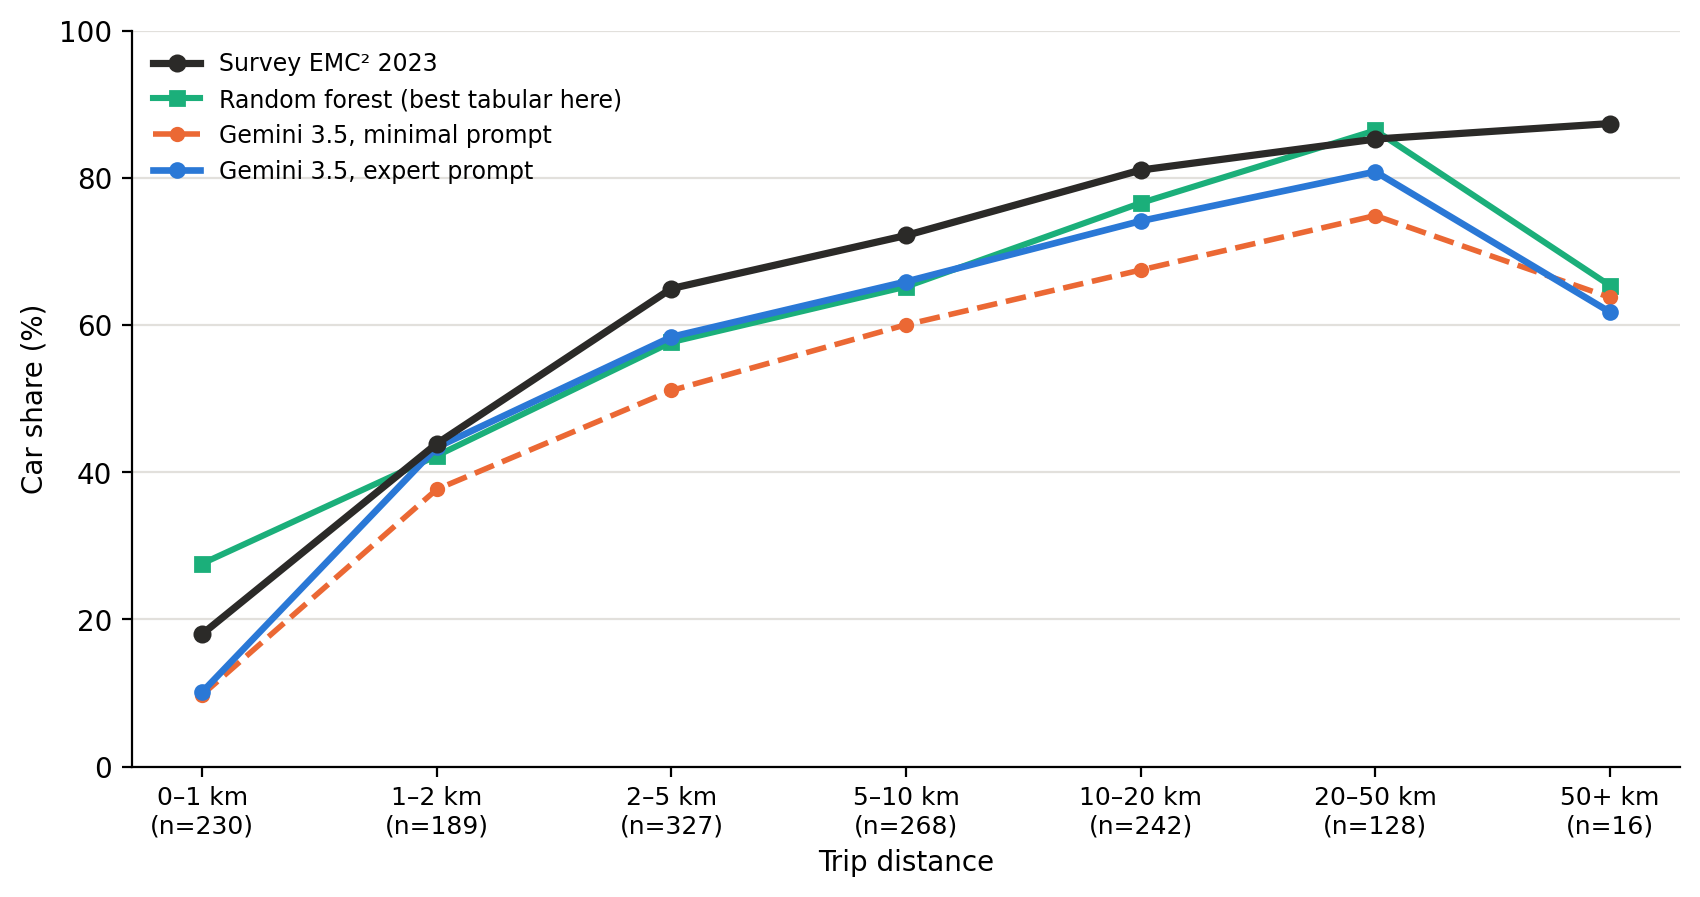
\includegraphics[width=0.78\columnwidth]{images/ch6_distance.png}
  \caption{The car share by distance band: the survey target, \texttt{gemini-3.5} under the minimal prompt then under the expert prompt, and the tabular method closest to the target on this dimension.}
  \label{fig:distance}
  \Description{A line chart. The x axis carries five distance bands, under one kilometre, one to three, three to ten, ten to fifty, and over fifty kilometres. The y axis is the car share in per cent, from zero to a hundred. The survey target rises steeply across the bands, from about eighteen per cent under one kilometre to about seventy-seven per cent beyond fifty. The curve for gemini-3.5 under the minimal prompt is almost flat, staying between forty and fifty per cent across every band, so it is far above the target on short trips and far below it on long ones. The curve for the same model under the expert prompt keeps the same low starting point, about eight points under the target under one kilometre, then rises band by band and ends eight to fourteen points higher than the minimal prompt at the long distances, which gives it a slope in the same direction as the target. A fourth curve shows the tabular method closest to the target on this dimension, the random forest, which tracks the target more closely at both ends.}
\end{figure}

\begin{figure*}[tp]
  \centering
  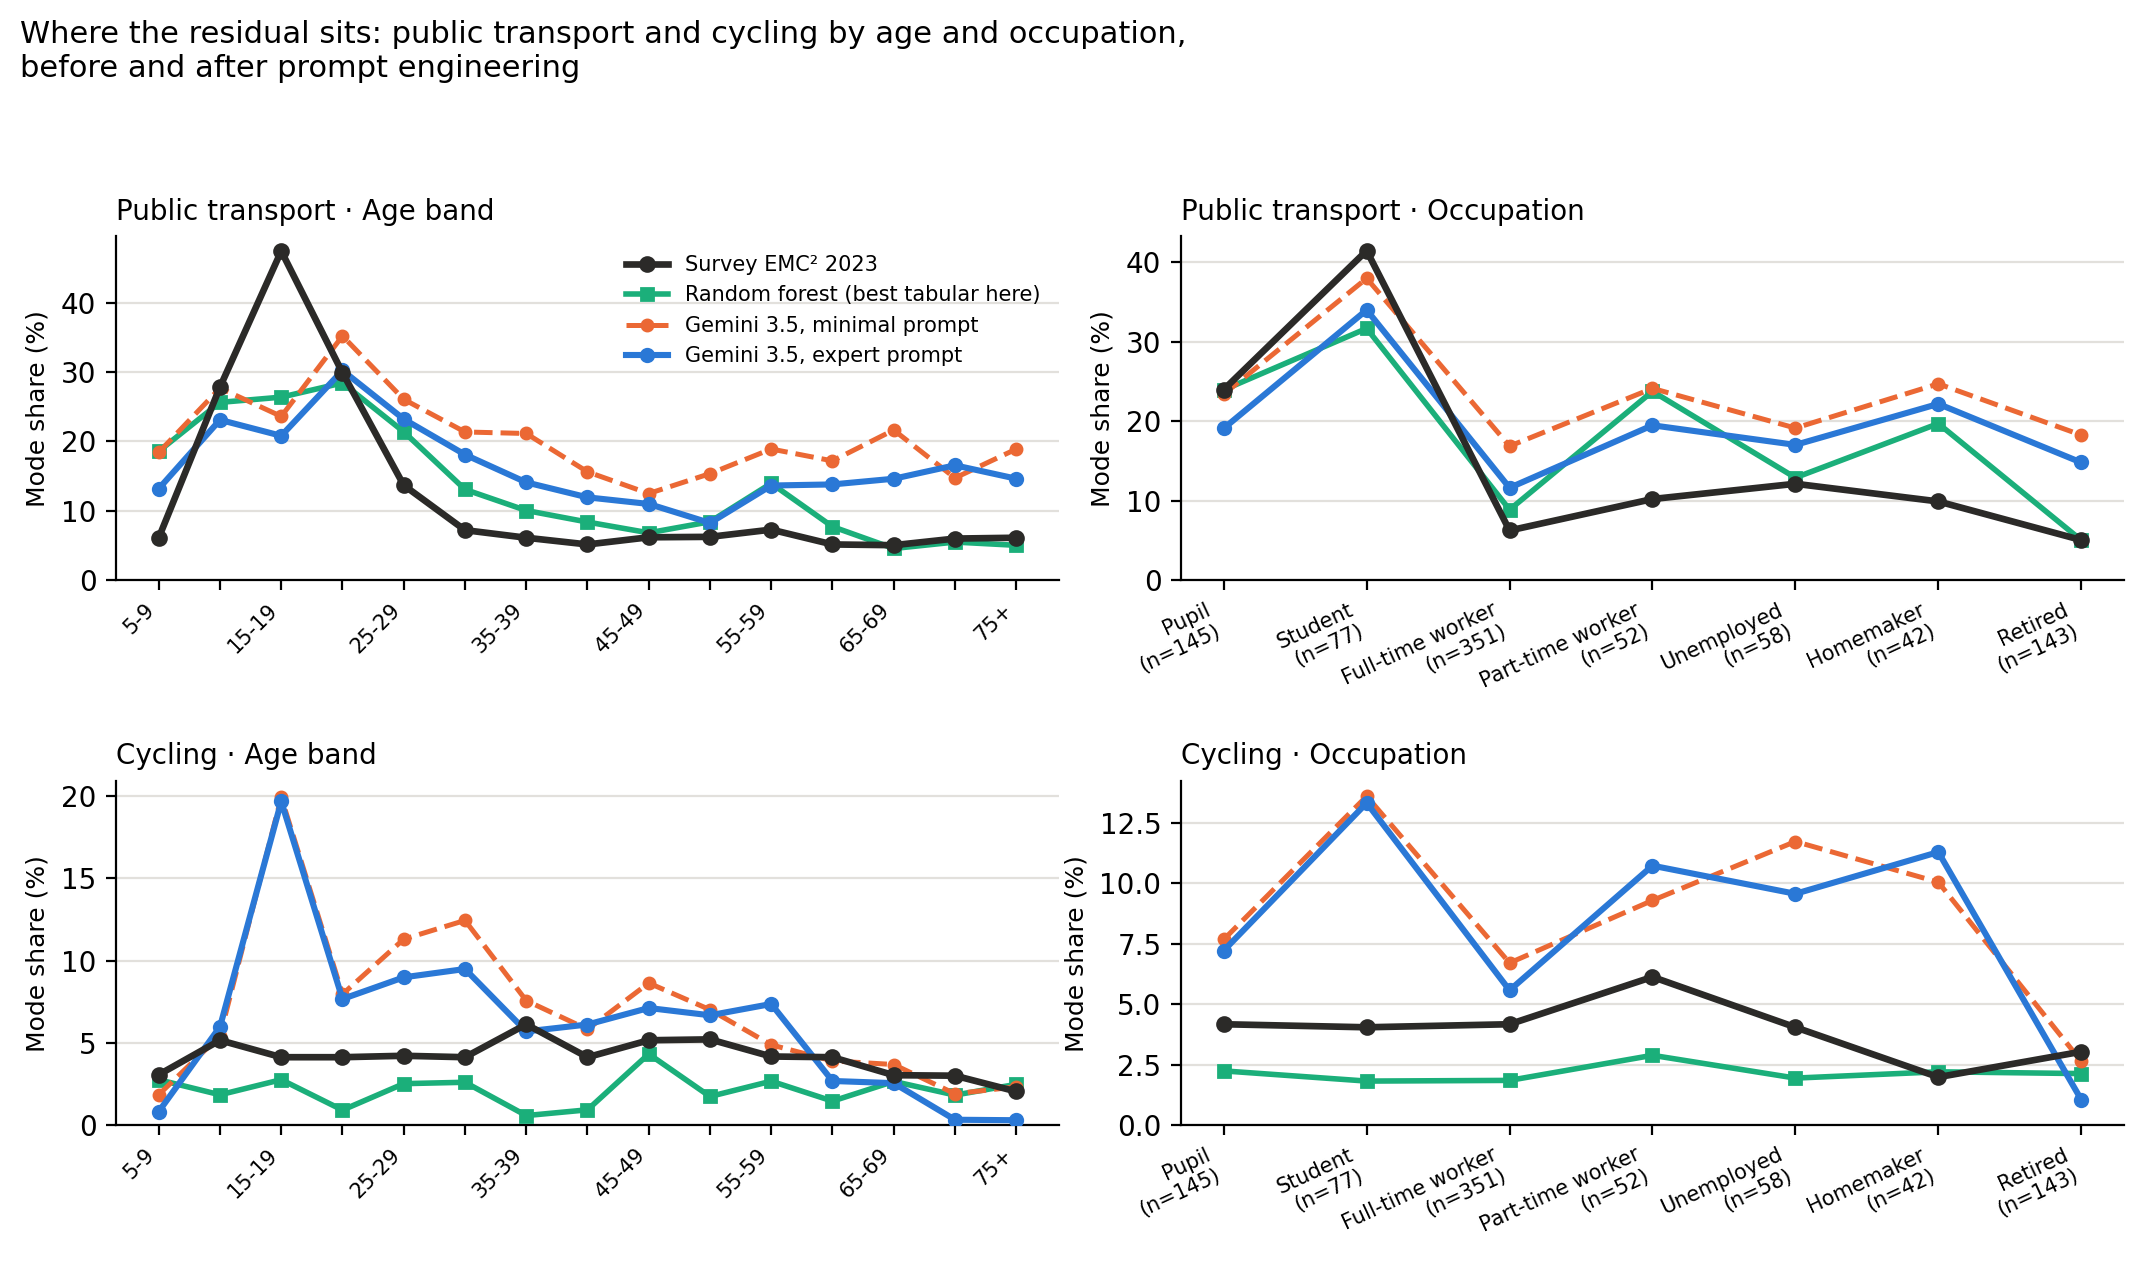
\includegraphics[width=\textwidth]{images/ch6_residu.png}
  \caption{The two modes that carry the residual, read by age and by occupation. The public transport peak of the 15--19 year olds, 47.4\,\% in the survey, is reproduced by no decider: the agent places 20.8\,\% there after tuning and the random forest 26.4\,\%. Cycling follows the opposite path on the same stratum, 19.7\,\% for the agent against 4.1\,\% observed, and tuning does not move it.}
  \label{fig:residual}
  \Description{Four bar panels in two rows. The top row carries public transport, the bottom row cycling; the left column reads by age band, the right column by occupation. In each panel, grouped bars compare the survey target, gemini-3.5 under the minimal prompt, the same model under the expert prompt, and the random forest. In the top-left panel the survey bar for the fifteen to nineteen year olds rises to 47.4 per cent, far above every other age band, while the agent reaches only 20.8 per cent after tuning and the random forest 26.4 per cent; the gap closes on the adult bands. The top-right panel repeats the pattern for school pupils and students. In the bottom-left panel the cycling bars are inverted: the agent places 19.7 per cent on the fifteen to nineteen year olds against 4.1 per cent observed, and the bar for the expert prompt is the same height as the bar for the minimal prompt, showing that tuning does not move this mode. The bottom-right panel shows the same excess for pupils and students.}
\end{figure*}

The two minority modes carry an error the instruction does not correct. The three language models place cycling between 6.8 and 8.1\,\% where the survey counts 4.1\,\%, and prompt engineering moves that share by only one tenth to eight tenths of a point, where it makes public transport fall back by four to eleven points: two errors coexist in the same decider, and only one answers the instruction. The two dimensions absent from the calibration cycle as from the composite, the residential ring and the housing type, are those where the agent falls furthest behind, by eight and by seven points against gradient boosting.

The detailed results are in Appendix~\ref{app:detail}: the error by dimension and by decider, the modal shares of each, the strata that tuning degrades on the three models, and four plates.

\subsection{Individual decision}
\label{sec:individual}

The unit accuracy announced in Section~\ref{sec:quantities} is measured on the days the respondents actually described, by the protocol of Section~\ref{sec:audit}: 9{,}621 trips made by 2{,}930 people, each carrying the mode they declared (Table~\ref{tab:unit}).

\begin{table}[tbp]
  \caption{Unit agreement on the declared trips, five deciders out of nine, in per cent except for cross-entropy, measured over the 5{,}451 decisions every decider compared scores. The other four and the precision columns are in Appendix~\ref{app:unit}.}
  \label{tab:unit}
  \small
  \setlength{\tabcolsep}{4pt}
  \begin{tabularx}{\columnwidth}{@{}Lrrrr@{}}
    \toprule
    Decider & \multicolumn{1}{c}{Acc.} & \multicolumn{1}{c}{Cross-} & \multicolumn{1}{c}{Bike} & \multicolumn{1}{c}{Walk} \\
            &    & \multicolumn{1}{c}{ent.} & \multicolumn{1}{c}{rec.} & \multicolumn{1}{c}{rec.} \\
    \midrule
    Gradient boosting & 71.5 & $\mathbf{0.299}$ & 20.4 & 63.4 \\
    Multinomial logit & 68.6 & 0.358 & 18.3 & 60.0 \\
    Shortest duration & 68.1 & ---   & 25.8 & 19.2 \\
    Expert prompt, \texttt{gemini-3.5}  & 67.6 & 0.342 & 22.5 & 47.2 \\
    Minimal prompt, \texttt{gemini-3.5} & 64.8 & 0.383 & 24.1 & 44.2 \\
    \bottomrule
  \end{tabularx}
\end{table}

The expert prompt names the declared mode slightly less often than the tabular methods. On cross-entropy, which weighs the probability a decider gave to the mode finally declared, it comes ahead of one of them alone, the multinomial logit. The ranking therefore depends on the quantity read without bringing the agent ahead, and neither of these two readings can be read off the composite of Section~\ref{sec:scale}, which compares aggregate shares alone.

\begin{figure*}[tp]
  \centering
  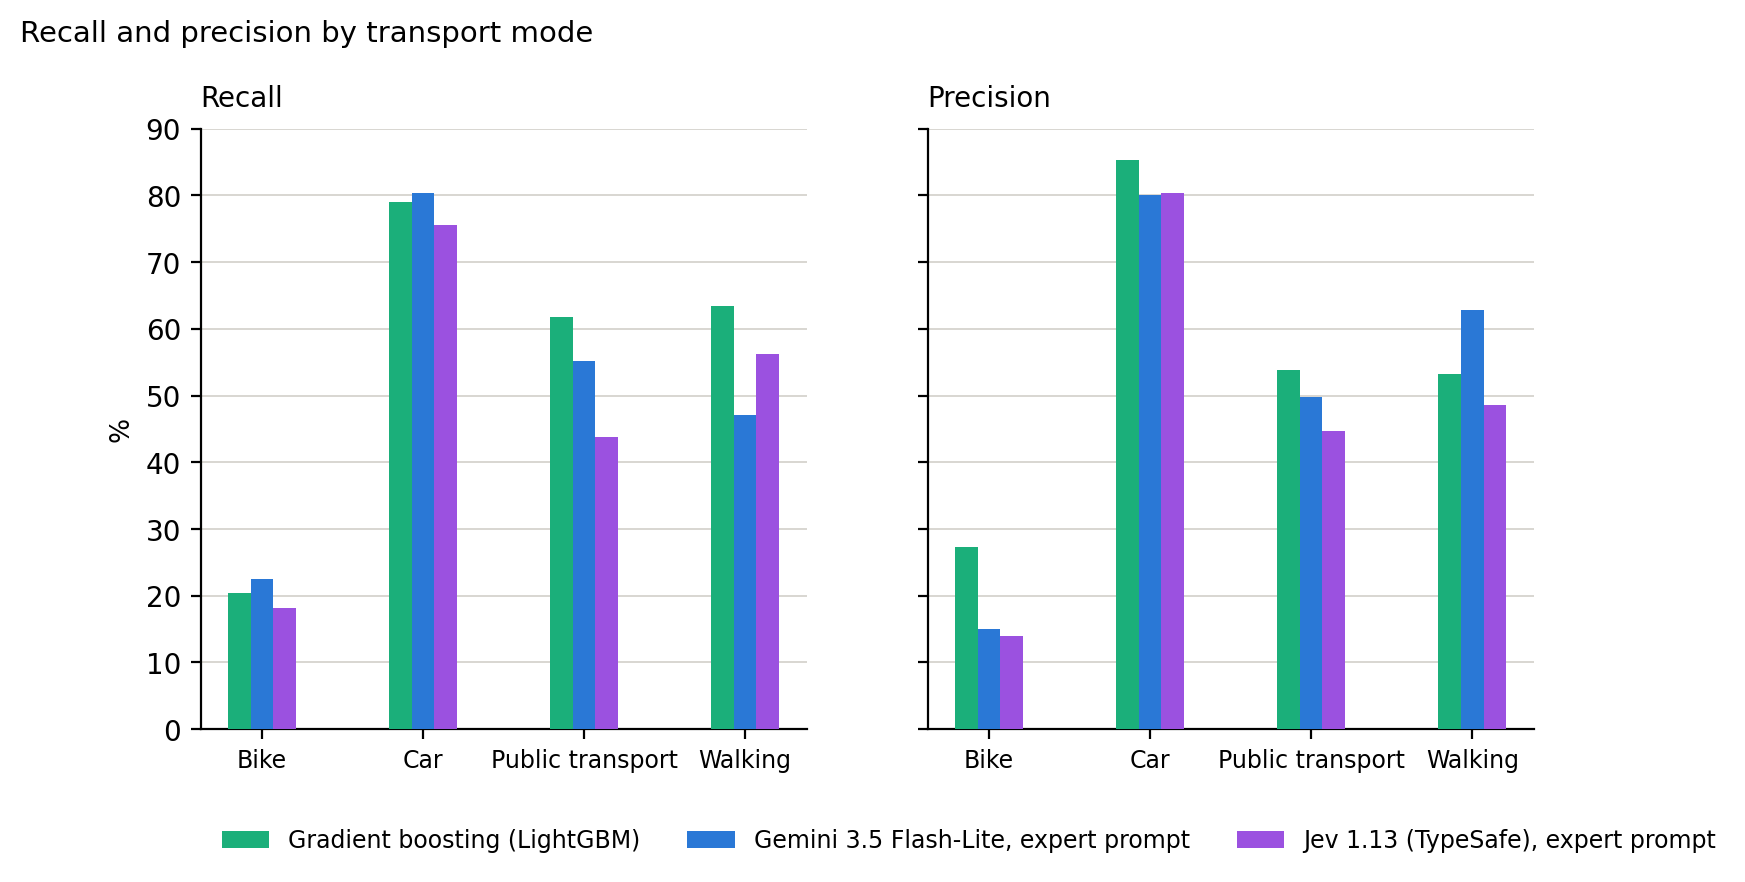
\includegraphics[width=\textwidth]{images/ch6_audit_modes.png}
  \caption{Recall and precision per mode, for the tabular ceiling and the two levels. Bikes are better recalled and less well predicted; walking goes to the car.}
  \label{fig:audit-modes}
  \Description{Two panels of grouped bars, recall on the left and precision on the right. In each panel the horizontal axis carries the four modes, bike, car, public transport and walking, and the vertical axis a percentage from zero to ninety. Three bars per mode: gradient boosting, the expert prompt and the minimal prompt. On the recall panel the two prompt bars stand above the gradient boosting bar on bike and below it on walking and public transport. On the precision panel the relation is reversed on those two modes: the prompt bars stand below gradient boosting on bike and above it on walking.}
\end{figure*}

% Figure « Unit agreement by distance band » retirée le 2026-09-22 à la demande de l'auteur.
% Le script scripts/analysis/plot_audit_unitaire.py produit toujours images/ch6_audit_distance.png.

The per-mode detail of the nine deciders, the confusion matrix and the ceiling of the audit are in Appendix~\ref{app:unit}.

\subsection{Cohort variation and between-seed dispersion}
\label{sec:dispersion}

A cohort of 1{,}000 personas measures a composite only to within $\pm 1.3$ points: that is the 95\,\% confidence interval obtained by resampling people with replacement, and it bounds what Table~\ref{tab:scale} allows to be told apart. The paired standard deviation of that term is about 0.7, so that no equivalence margin below 1.4 points will be concluded from one run on this cohort; only further cohorts lower it. This is why every comparison in this section is paired: playing the two deciders on the same personas makes that term act on both sides, where it cancels.

Between-seed dispersion, for its part, leaves the gaps of this section where they are. Replayed on the same cohort with other seeds, a language-model decider stays within cohort variation, and none of the paired differences of Sections~\ref{sec:scale} and~\ref{sec:engineering} changes sign.

% REVIEW WARNING: the two claims of the paragraph above anticipate a result that is NOT yet measured, and carry a **TBC**
%   in the Markdown master. Author's decision of 2026-09-17: write the chapter taking between-seed dispersion as given and
%   similar, and lift the TBC when ticket 073 axis 1 has delivered its identical replay. No figure is advanced while the
%   measurement does not exist. Do not publish this paragraph without that replay.

Two measurements already give the order of magnitude. The same prompt, on the same model and with the same seed, replayed on a corrected substrate, moves its composite by 0.24 to 1.17 points depending on the decider, where deterministic deciders move by less than 0.12; and two runs of the same prompt on two successive cohorts agree on 86.1\,\% of the most likely modes. Both confound the non-determinism of the model with the change of substrate, and it is identical replay that separates them.

% NO FLOAT FLUSH HERE. \afterpage{\clearpage} stood here until 2026-09-21 and broke the
%   compilation (see 03_Architecture.tex). Ten floats for less than one page of running text,
%   six of them full width, about 1,760 pt of double-column matter where a page offers at most
%   0.85 * 662 pt of top area: the queue drains at its own pace and the plates land where LaTeX
%   can place them, chapters 7 to 9 included.
%   THE MASS IS THE PROBLEM, not the flush: as long as ch6_echelle, ch6_residu, ch6_audit_modes
%   were all figure*, chapter 6 carried three or four pages of near-solid figures. Le retrait de
%   ch6_audit_distance le 2026-09-22 en rend une ; demoting ch6_audit_modes to single column, or moving one plate
%   to the appendix, is the only thing that changes that. Author's call, not made here.
